\chapter{Vlastní řešení}  

V této části navrhneme podobu vlastního řešení problému specifikovaného v předchozích kapitolách. Návrh by měl nabízet jednoduché a vyhovující řešení vycházející ze stanovených požadavků a cílů. 

\section{Návrh}

Cílem práce je poskytnout konverzi \LaTeX\ souborů do PDF, čehož bude dosaženo pomocí webové služby. Tato služba bude poskytovat svoje rozhraní a funkcionalitu portálům Moodle a CourseWare. Jedná se o jednoduchou aplikaci s jediným účelem, tedy kompilace \LaTeX\ souborů do PDF. Tudíž není potřeba složité databáze, ale stačí pouze SQLite\footnote{https://www.sqlite.org/}, což je velmi odlečená verze klasických SQL databází, která ukládá data přímo do souboru v souborovém systému, kam bude ukládán i výsledný soubor PDF. 

\subsection{Platforma}
Na základě požadavků bude aplikace postavena na Java EE, což je platforma pro vývoj webových aplikací rozšiřující standardní Javu SE. Oproti ní poskytuje některé zásadní techniky navíc, jednu si tedy představme. 
\par
\textbf{Vkládání závislostí} (dependency injection) umožňuje objektu používat jiné objekty bez potřeby ho zatěžovat jejich vytvářením. Objekty, které můžeme takto vkládat, se nazývají beany a právě o jejich vytváření a zánik se stará Contexts and Dependency Injection (dále jen CDI) kontejner.
\\[12pt]
\par
Dále je potřeba specifikovat aplikační server. Ten poskytuje pro webové aplikace běhové prostředí, tedy zajišťuje správu databázových spojení apod. Na základě zkušeností je vybrán open-source Payara, který staví na GlassFish, oproti němu poskytuje častější aktualizace a opravy chyb. 

\subsection{Architektura}
Architektura popisuje z jakých částí se aplikace skládá, jak mezi sebou tyto části komunikují a jakým způsobem procházejí informace a požadavky aplikací. Při navrhování architektury je potřeba zvážit několik věcí, například rozšířitelnost, modularizaci, odezva a složitost. 
\par
Nejpoužívanšjší architekturou u webových aplikací je klient-server architektura s n vrstvami, která aplikaci rozděluje na n fyzických médií a n vrstvá architektura, která označuje n logických celků.\footnote{V anglických zdrojích se používají výrazy N-Tier Client-Server architecture a N-Layered architecture, kde tier znamená to samé jako layer, tudíž vrstva} Nejčastěji jsou obě architektury 3 vrstvé, tedy rozdělení je následující: prezentační, aplikační a databázová vrstva. Ovšem služba, kterou se zabýváme v této práci nemá uživatelské rozhraní a vystavuje jenom určité API, tudíž odpadá prezentační vrstva. Ani neobsahuje databázový server, zůstává tedy jenom aplikační fyzická vrstva, což z naší služby dělá jedno-vrstvou klient-server aplikaci. Zbývá ještě vyřešit logickou architekturu, kde se budeme držet také zavedeých postupů, ale zbavíme se prezentační vrstvy a zůstane nám 2-vrstvá architektura obsahující byznys logiku a přístup k databázi.  

\begin{figure}[H]
	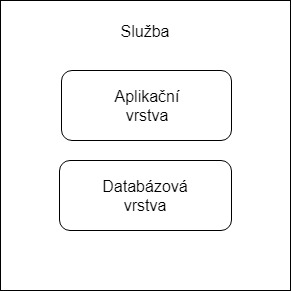
\includegraphics[scale=0.7]{architecture}
	\centering
	\caption{Architektura}
	\label{fig:arch}
\end{figure}

\subsection{Komunikace}
Pro komunikaci mezi klientem a serverem je vybráno REST Api. Poskytuje jednoduché rozhraní, se kterým je schopen komunikovat jakýkoliv systém pouze na základě znalosti struktury požadavků a odpovědí. Posílání zpráv bude postaveno nad protokolem HTTP pomocí GET a POST metod. Na obrázku \ref{fig:seq} je zobrazena komunikace mezi serverem a klientem. 

\begin{figure}[H]
	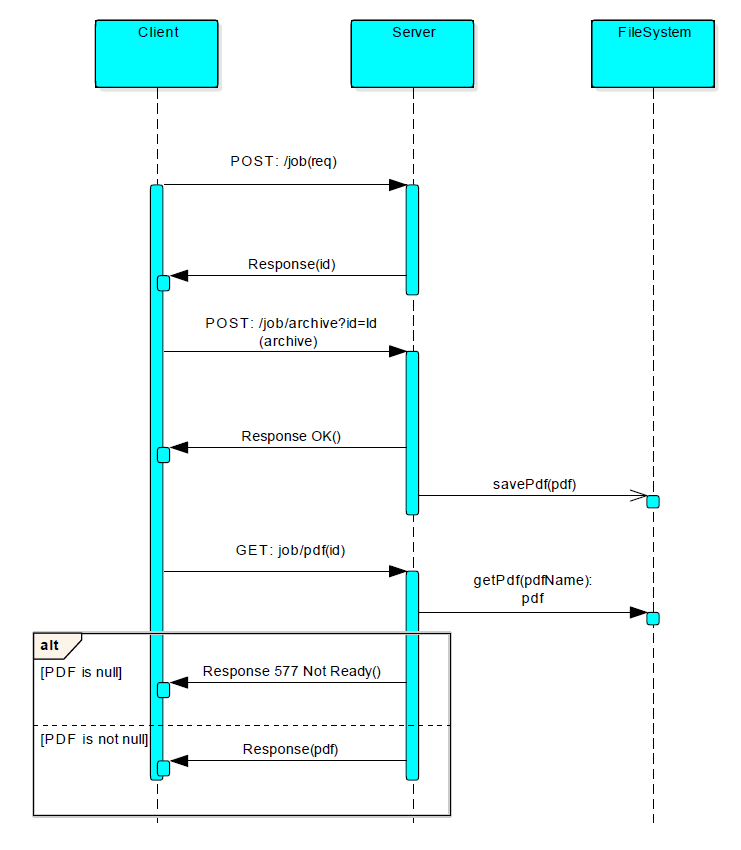
\includegraphics[width=0.9\textwidth]{diagram}
	\centering
	\caption{Sekvenční diagram}
	\label{fig:seq}
\end{figure}

Kompletní dokumentace k rozhraní se nachází na swagger\footnote{https://app.swaggerhub.com/apis/Tadky/Thesis/1}. Na ukázku vypíšeme alespoň používané zdroje:
\begin{itemize}
	\item \textbf{POST} {\ttfamily /job} - Slouží k předání požadavků na výsledné PDF.
	\item \textbf{POST} {\ttfamily /job/archive?id=<jobId>} - Musí obsahovat zip archiv s potřebnými soubory pro kompilaci.
	\item \textbf{GET} {\ttfamily /job/pdf?id=<jobId>} - Vrací výsledné PDF, pokud už je hotové.
	\item \textbf{HEAD} {\ttfamily /job/pdf?id=<jobId>} - Odpověď obsahuje pouze hlavičku, která informuje o stavu PDF
	\item \textbf{GET} {\ttfamily /info} - Slouží k získání informací ohledně serveru, tedy verze kompilátoru, operačního systému, zbývajícího volného místa na disku
\end{itemize}
Všechny tyto zdroje navíc obsahují parametr\footnote{Typ parametru, který se posílá v samotné URL daného dotazu ve formě klíč=hodnota} token, který zajišťuje autentizaci. Ta je rozebrána v další sekci.

\subsection{Zabezpečení}
Zabezpečení bude zavedeno jenom v minimální míře pomocí statických tokenů, které budou mít dané portály pro sebe k dispozici. Vzhledem k povaze dat není nutné používat OAuth\footnote{Protokol pro autentizaci a autorizaci aplikací.} server, jehož implementace by byla značně nad rámec mé práce. Tokeny budou sloužit k autentizaci portálů, jímž budou tokeny vygenerovány a předány jejich správcům. Každá zpráva poslaná na server bude obsahovat token, který se bude ověřovat oproti tokenu uloženém v properties\footnote{Soubor v němž jsou data uspořádány klíč = hodnota} souboru. Token bude posílán v parametru dotazu v otevřené formě. 

\subsection{Kompilace}
Pro vytvoření PDF je nutné příslušně zkompilovat celý \LaTeX\ projekt. Pro úspěšnou kompilaci je potřeba, aby kompilátor měl k dispozici všechny balíčky, které jsou použity v projektu. Jsou tři způsoby, jak toho docílit.
\begin{enumerate}
	\item Stáhnout všechny balíčky již při instalaci kompilátoru
	\item Nainstalovat čistý kompilátor
		\begin{enumerate}
			\item Stáhnout několik balíčků a jenom ty se budou používat
			\item Získávat balíčky podle potřeby za běhu
		\end{enumerate}
\end{enumerate}
První možnost je zbytečná z důvodu mnoha nepoužívaných balíčků a velikosti na disku. Druhá možnost nabízí dvě podmožnosti, kde volba s přednastavenými balíčky vytváří omezení pro uživatele tudíž je může odrazovat od používání aplikace. Nejvíce vhodná se zdá poslední možnost, která eliminuje všechny neduhy předchozích, tím pádem je i zvolena.
\par
Na základě porovnání kompilátorů (sekce \ref{compilator}) z předchozí kapitoly je zvolen MikTeX, který poskytuje vše potřebné a nabízí vhodné funkcionality pro téma této práce např. doinstalovávání balíčku za běhu. Bude nainstalován ve verzi \enquote{Just enough TeX}, tudíž nebude obsahovat žádné balíčky. Ty se právě budou doinstalovávat až na požadavek při kompilaci.

\subsection{PDF úpravy}
Jelikož jsou kladeny požadavky na výsledný soubor PDF a bohužel kompilátory tyto úpravy nepodporují, je potřeba použít jiný nástroj, který bude umožňovat měnit soubor podle požadavků. Nejvíce vhodný se zdá PDFtk\footnote{https://www.pdflabs.com/tools/pdftk-server/}, který je pod GPL\footnote{Poskytuje svobodu šíření, provozování a upravování daného software.} licencí a nabízí vše potřebné. Tedy po zkompilování do PDF se za pomoci výše zmíněné aplikace aplikují požadavky, které byly obdrženy od klienta.

\subsection{Server}
V této fázi návrhu máme už všechny potřebné informace, aby mohl být zvolen operační systém a stanoveny požadavky na server. Jsou známy dvě omezující podmínky kladené na systém. První vychází z požadavků: operační systém musí být Debian nebo CentOS. Druhou určuje kompilátor. Jelikož byl zvolen MikTeX, který je podporován na Debian a Ubutnu, volba je jednoznačná. Na základě průniku je vybrán nejnovější Debian, tedy verze 9 s označením \enquote{stretch}. 
\par
Je také potřeba stanovit velikost diskového pole potřebného pro fungování. Jelikož nejvíce místa budou zabírat balíčky a potažmo výsledné pdf, budeme vycházet hlavně z těchto údajů. Přibližná velikost všech balíčků obsažených v plné verzi kompilátoru je zhruba 4GB, což bylo zjištěno na základě testovací instalace. Dále je potřeba odhadnout velikost všech PDF, které musí server uchovávat po dobu jednoho měsíce, v jeden moment. Horní odhad pro počet vytvořených PDF za den je 30 a pro velikost souboru je 10MB. Tedy na konci měsíce se může očekávat velikost cca 10GB. Tedy celkové požadované místo je 15GB.  
 



